\documentclass[t]{beamer}
\usetheme{Warsaw}
\usecolortheme{seahorse}
\usepackage{array}
%\usepackage{graphicx}
\usepackage{amssymb,amsmath,mathrsfs,amsfonts}
%\usepackage[colorhighlight,display]{texpower}
%\usepackage{caption}
%\usepackage[all]{xy}
\usepackage{beamerthemesplit}
\mode<presentation>
%\usepackage{pause}
\usepackage{ulem}  % for strikethroughs
\usepackage{cancel} % for strikethroughs in math mode 
\usepackage{tikz}
\usepackage{calc}
\usetikzlibrary{shapes}
\usepackage{hyperref}
\hypersetup{pdfpagemode=FullScreen}
\usepackage{ifthen}
\usepackage{animate}
\usepackage{color}
\usepackage{type1cm}  % used for watermarking
\usepackage{eso-pic}  % used for watermarking

\usepackage[font={footnotesize}]{caption}



\theoremstyle{plain}
\newtheorem{prop}{Proposition}
\newtheorem{thm}[prop]{Theorem}
\newtheorem{lem}[prop]{Lemma}
\newtheorem{cor}[prop]{Corollary}
\theoremstyle{definition}
\newtheorem{dfn}{Definition}
\newtheorem{rem}[prop]{Remark}
\newtheorem{ex}{Example}[section]
%\newtheorem{note}{Note}[section]
\newtheorem{exercise}{Exercise}[section]
\newcommand{\nin}{\noindent}
\newcommand{\ds}{\displaystyle}
\renewcommand{\figurename}{Figure \arabic{figure}}



\renewcommand*\familydefault{\sfdefault} 




%%%%%%%%%%%%%%%%%%%%%%%%%%5
%%%%%%%%%%%%%%%%%%%%%%%%%%%%
%%%% some commands that have different meaning in the article/presentation modes

\newcommand{\vvfill}{\mode<presentation>{\vfill}  \mode<article>{\medskip}}   %vfill in presentation only
\newcommand{\sketchspace}{ 
\mode<article>{ \medskip\noindent{\textbf{Sketch:}} \vspace*{6cm} }
\mode<presentation>{ } 
}
\newcommand{\examplespace}{ 
\mode<article>{ \medskip\noindent{\textbf{Example:}} \vspace{6cm} }
\mode<presentation>{ } 
}
\newcommand{\artsmspace}{\mode<article>{\vspace*{2cm}} }  %small space in article mode
\newcommand{\artlargespace}{\mode<article>{\vspace*{6cm}} }  %large space in article mode

\newcommand{\dx}{\,dx}

\newcommand{\soln}{{\textbf{Solution: }}\,\,\,}
\newcommand{\disp}{\displaystyle}

\newcommand{\makedate}{\vvfill
\begin{picture}(10,10)  
\put(260,-20){\mbox{\tiny{\today}}}
\end{picture}
}

\newcommand{\pd}[2]{\dfrac{\partial#1}{\partial#2}}
\newcommand{\pD}[2]{\dfrac{\partial^2#1}{\partial#2^2}}
\newcommand{\pdd}[3]{\dfrac{\partial^2#1}{\partial#2 \partial#3}}


\normalem %stops the ulem package making all the emphs into underlines....
 
 
 
 \newcommand{\refandrev}[2]{
 \begin{small}
  \hspace{6cm}
  \begin{minipage}[r]{8cm}
  Stewart,    Chapter #1   \\
  Review:  \parbox[t]{6cm}{#2}
\end{minipage}
\end{small}
}



\newcounter{heading}
\setcounter{section}{1}
\setcounter{heading}{0}

\newcommand{\makeheading}[1]{\medskip\begin{large}\noindent\textbf{{#1}}\end{large}\smallskip}

%\newenvironment{head}[1]{\medskip\stepcounter{heading}\noindent\textbf{\hspace{0.2cm}{#1}.}}{}
\newcommand{\newhead}[1]{\medskip\stepcounter{heading}\noindent\textbf{\hspace{0.2cm}{#1}.}}


\newcommand{\pf}[1]{\noindent\textit{Proof.}\vspace*{#1 cm}}
\newcommand{\sol}[1]{\noindent\textit{Solution.}\vspace*{#1 cm}}
\newcommand{\further}[1]{\begin{small}\noindent\textit{Further reading: #1}\end{small}}
\newcommand{\exr}[1]{\begin{footnotesize}\noindent\textit{\textbf{Exercises:} Stewart #1}\end{footnotesize}}


% Sets of numbers
\newcommand{\C}{\mathbb{C}}
\newcommand{\RR}{\mathbb{R}}
\newcommand{\Z}{\mathbb{Z}}
\newcommand{\N}{\mathbb{N}}
\newcommand{\Q}{\mathbb{Q}}

% Partitions
\newcommand{\PP}{\mathcal{P}}

% Limits
\newcommand{\limm}[1]{\displaystyle \lim_{x\to #1}}

% Backslash
\newcommand{\bs}{\backslash}

% functions
\newcommand{\cosec}{\mathrm{cosec}}
\newcommand{\cosech}{\mathrm{cosech}}
\newcommand{\sech}{\mathrm{sech}}
\newcommand{\Li}{\mathrm{Li}}
\newcommand{\si}{\mathrm{Si}}
\newcommand{\erf}{\mathrm{erf}}

% Domain and Range
\newcommand{\Dom}{\mathrm{Dom}}
\newcommand{\Codom}{\mathrm{Codom}}
\newcommand{\Range}{\mathrm{Ran}}



\title{Week 5:  Approximation}

\begin{document}

\frame{\titlepage}

\setcounter{tocdepth}{2}
\frame{\tableofcontents
}

\AtBeginSection[]
{
\begin{frame}<beamer> 
\tableofcontents[currentsection]  % show TOC and highlight current section
\end{frame}
}

\section{Linear Approximation}

\frame
{
\frametitle{Linear Approximation}

\begin{dfn}
We could use tangent line at $x=a$ to predict $f(x)$.
\centering
$L(x) = f(x) \approx f(a) + f'(a)(x-a)$
\vspace{0.2em}
\end{dfn}

\begin{figure}[t]
\begin{center}
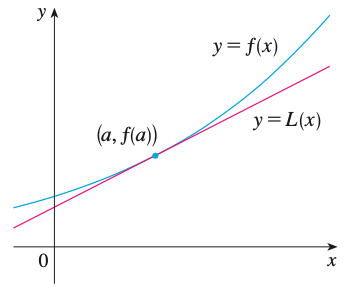
\includegraphics[scale=0.4]{fig/linearapprox}
\end{center}
\end{figure}

}

\begin{frame}

\frametitle{Example}

Find the linearization of the function $f(x) = \sqrt{x + 3}$ at $a=1$ and use it to approximate the numbers $\sqrt{3.98}$ and $\sqrt{4.05}$.  \pause

\begin{itemize}
	\item $f'(x) = \dfrac{1}{2\sqrt{x+3}}$
	\item So we have $f(1) = 2$ and $f'(1) = \dfrac{1}{4}$
	\item Putting into the linearization equation, we get $L(x) = f(1) + f'(1)(x-1) = 2 + \dfrac{1}{4}(x-1) = \dfrac{7}{4} + \dfrac{x}{4}$
	\item Thus $\sqrt{x+3} \approx \dfrac{7}{4} + \dfrac{x}{4}$
	\item For $\sqrt{3.98}$,  $\sqrt{3.98} \approx \dfrac{7}{4} + \dfrac{0.98}{4} = 1.995$
	\item For $\sqrt{4.05}$,   $\sqrt{4.05} \approx \dfrac{7}{4} + \dfrac{1.05}{4} = 2.0125$
\end{itemize}

\end{frame}

\begin{frame}

\frametitle{Example}

Use linear approximation to estimate $\sqrt{59}$ without a calculator.  \pause

\begin{itemize}
	\item Let $f(x) = \sqrt{x}$
	\item Let $a = 64$ since $\sqrt{64}$ is easy
	\item $f'(x) = \dfrac{1}{2\sqrt{x}}$
	\item So we have $f(64) = 8$ and $f'(64) = \dfrac{1}{16}$
	\item Putting into the linearization equation, we get $L(x) = f(64) + f'(64)(x-64) = 8 + \dfrac{1}{16}(x-64) = 4 + \dfrac{x}{16}$
	\item Thus $\sqrt{x} \approx 4 + \dfrac{x}{16}$
	\item For $\sqrt{59}$,  $\sqrt{59} \approx 4 + \dfrac{59}{16} = 7.6875$
\end{itemize}

\end{frame}

\begin{frame}

\frametitle{Exercise}

Find the linear approximation of the function $f(x) = \sqrt{1-x}$ at $a=0$.  Then use it to approximate the numbers $\sqrt{0.9}$ and $\sqrt{0.99}$.  \pause

\begin{itemize}
	\item $f'(x) =- \dfrac{1}{2\sqrt{1-x}}$
	\item So we have $f(0) = 1$ and $f'(0) = -\dfrac{1}{2}$
	\item Putting into the linearization equation, we get $L(x) = f(0) + f'(0)(x-0) = 1 + -\dfrac{1}{2}(x-0) = 1 - \dfrac{1}{2}x$
	\item Thus $\sqrt{0.9} = \sqrt{1-0.1} \approx1 - \dfrac{1}{2}(0.1) = 0.95$
	\item Thus $\sqrt{0.99} = \sqrt{1-0.01} \approx1 - \dfrac{1}{2}(0.01) = 0.995$
\end{itemize}

\end{frame}

\section{Differential Approximation}

\frame
{
\frametitle{Differential Approximation}

\footnotesize

\begin{dfn}
Given $\dfrac{dy}{dx} = f'(x)$, we know $dy = f'(x)dx$.      On a given graph below, let $dx = \Delta{x}$.  The corresponding change in $y$ is $\Delta{y} = f(x + \Delta{x}) - f(x)$.     The $dy$ is the amount in which the tangent line rises, while $\Delta{y}$  is the amount in which $y=f(x)$ falls.   Many times, $dy$ can be used to approximate $\Delta{y}$.
\end{dfn}

\begin{figure}[t]
\begin{center}
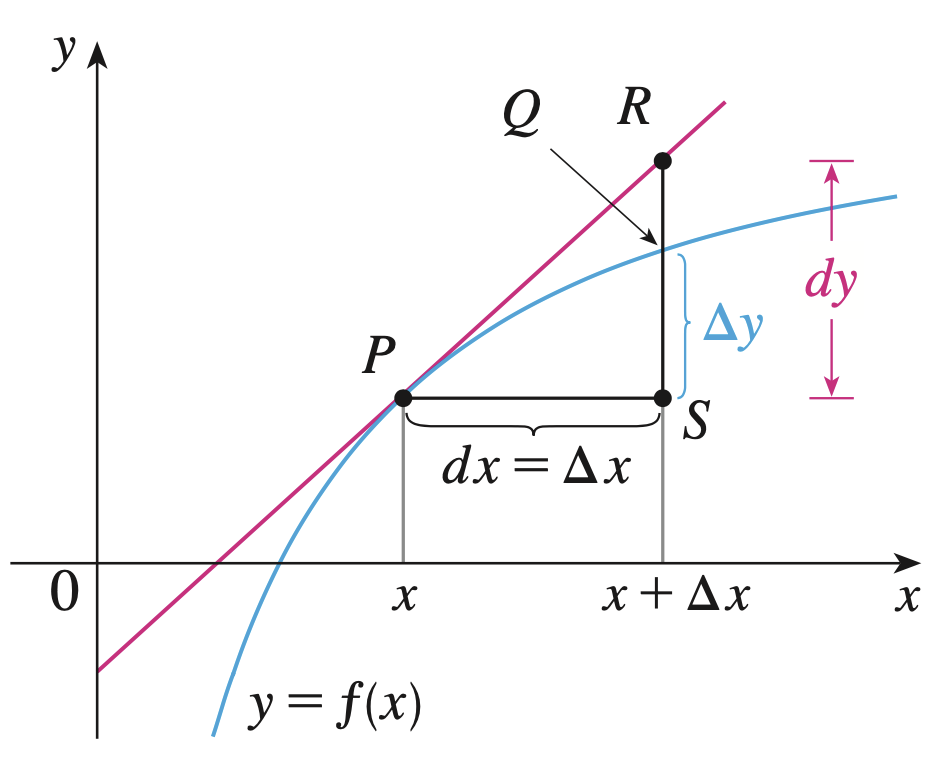
\includegraphics[scale=0.27]{fig/differentials}
\end{center}
\end{figure}

}

\begin{frame}

\frametitle{Example}

Compare the values of $\Delta{y}$ and $dy$ if $y=f(x) = x^3 + x^2 - 2x + 1$ and $x$ changes from 2 to 2.05 \pause

\begin{itemize}
	\item $f(2) = 2^3 + 2^2 - 2(2) + 1 = 9$
	\item $f(2.05) = 2.05^3 + 2.05^2 - 2(2.05) + 1 = 9.717625$
	\item $\Delta{y} = f(2.05) - f(2) = 0.717625$
	\item $dy = f'(x)dx = (3x^2 + 2x - 2)dx$
	\item Given $x=2$ and $dx = 0.05$, $dy = (3(2)^2 + 2(2) -2)0.05 = 0.7$
\end{itemize}

We can see that $dy$ can be used to approximate $\Delta{y}$.

\end{frame}

\begin{frame}

\frametitle{Exercise}

Compare the values of $\Delta{y}$ and $dy$ if $y=f(x) = x^3 + x^2 - 2x + 1$ and $x$ changes from 2 to 2.01 \pause

\begin{itemize}
	\item $f(2) = 2^3 + 2^2 - 2(2) + 1 = 9$
	\item $f(2.01) = 2.01^3 + 2.01^2 - 2(2.01) + 1 = 9.140701$
	\item $\Delta{y} = f(2.01) - f(2) = 0.140701$
	\item $dy = f'(x)dx = (3x^2 + 2x - 2)dx$
	\item Given $x=2$ and $dx = 0.01$, $dy = (3(2)^2 + 2(2) -2)0.01 = 0.14$
\end{itemize}

We can see that $dy$  is closer to $\Delta{y}$ as $dx$ gets smaller.  For more complicated functions, it may not be possible to compute $\Delta{y}$ thus such approximation is useful.

\end{frame}

\section{L'Hospital's Rule}

\begin{frame}
\frametitle{Indeterminant Forms}

\footnotesize

\noindent The limits of the form $\frac{\infty}{\infty}$ (also called `\textit{indeterminate forms}') that we studied so far can be calculated using algebraic trick.   What about the following limits?
\[\lim_{x\to\infty}\frac{e^x}{x} \qquad\qquad\qquad \ds\lim_{x\to\infty}\frac{\ln x}{x}\]

\noindent One way to solve this problem is to use the derivative. 

\begin{figure}[t]
\begin{center}
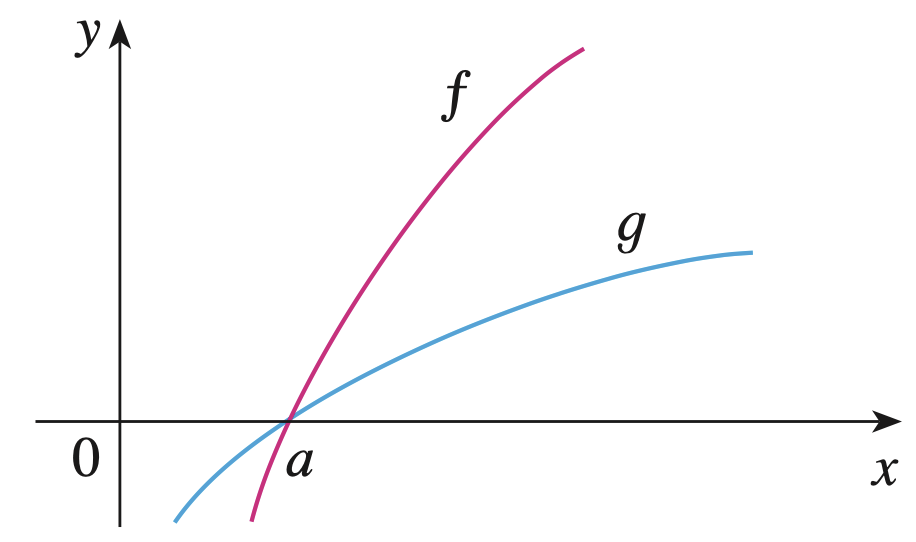
\includegraphics[scale=0.2]{fig/hospital1}
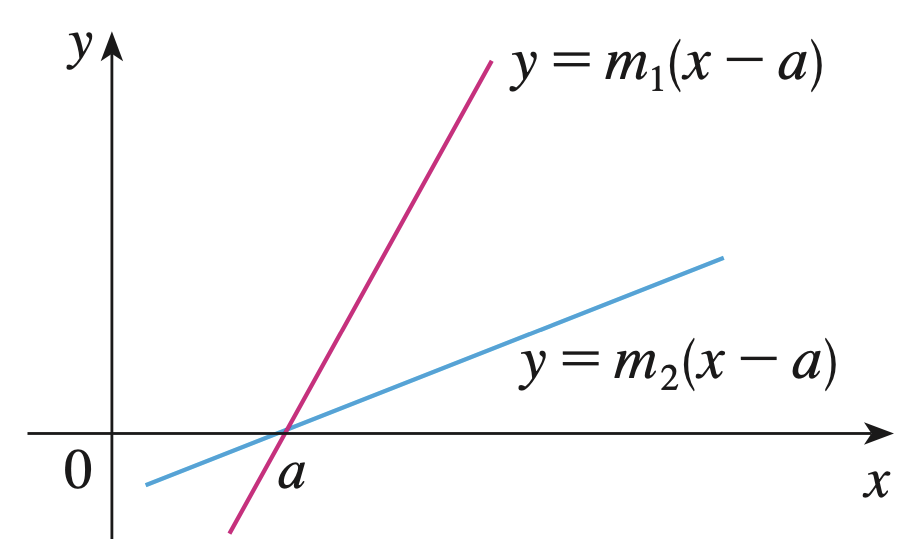
\includegraphics[scale=0.2]{fig/hospital2}
\caption{If we zoom in toward the point $(a, 0)$, the graphs would start to look almost linear.  If the graph is actually linear, their ratio would be $\dfrac{m_1(x-a)}{m_2(x-a)} = \dfrac{m_1}{m_2}$ which is the ratio of their derivatives.  Thus  $\limm{a}\dfrac{f(x)}{g(x)} = \limm{a}\dfrac{f'(x)}{g'(x)} $}
\end{center}
\end{figure}


\end{frame}

\subsection{Quotient}

\begin{frame}
\begin{block}{L'H\^opital's rule}
Suppose that $f$ and $g$ are differentiable functions, $a \in \mathbb{R}$, and $g'(x) \neq 0$, except possibly at $a$. Suppose also that either one of the two following conditions hold:
\begin{itemize}
\item $f(x)\to0$ and $g(x)\to0$ as $x\to a$;
\item $f(x)\to\pm\infty$ and $g(x)\to\pm\infty$ as $x\to a$.
\end{itemize}
If
\[\limm{a}\frac{f'(x)}{g'(x)}\]
exists or is $\pm \infty$, then
\[\limm{a}\frac{f(x)}{g(x)}=\limm{a}\frac{f'(x)}{g'(x)}.\]
\end{block}


\end{frame}

\begin{frame}
\newhead{Remarks}
\begin{enumerate}
\item[(i)] The theorem also holds for limits at infinity or one-sided limits, That is,  as $x\to\infty$ or $x\to-\infty$, or  $x\to a^+$ or as $x\to a^-$.
\item[(ii)] When using L'Hospital's Rule, we \textbf{do not} use the quotient rule.  We differentiate the numerator and the denominator \textbf{separately}.
\item[(iii)] Be sure to verify that the hypotheses in L'Hospital's rule are satisfied before applying it!
\item[(iv)] The rule can be applied multiple times.
\item[(v)] Can convert the rule for indeterminate form in products, differences, or powers.
\end{enumerate}
\end{frame}


\begin{frame}

\frametitle{Example}

Solve $\limm{1}\ds\frac{\ln x}{x-1}$

This is an indeterminate form of type $\dfrac{0}{0}$  \pause

\begin{itemize}
	\item $\limm{1}\ds\frac{\ln x}{x-1} = \limm{1}\ds\frac{\dfrac{d}{dx}\ln x}{\dfrac{d}{dx}(x-1)}$
	\item $\limm{1}\ds\frac{\dfrac{1}{x}}{1} $
	\item $\limm{1}\ds\frac{1}{x} = 1$
\end{itemize}

\end{frame}

\begin{frame}

\frametitle{Example}

Solve $\limm{\infty}\ds\frac{e^{x}}{x^{2}}$

This is an indeterminate form of type $\dfrac{\infty}{\infty}$  \pause

\begin{itemize}
	\item $\limm{\infty}\ds\frac{e^{x}}{x^{2}}= \limm{1}\ds\frac{\dfrac{d}{dx}e^{x}}{\dfrac{d}{dx}x^{2}} = \limm{\infty}\dfrac{e^{x}}{2x}$
\end{itemize}

We still get indeterminate form of  $\dfrac{\infty}{\infty}$.   Apply the rule again! 

\begin{itemize}
	\item $ \limm{\infty}\dfrac{e^{x}}{2x} = \limm{\infty}\dfrac{e^{x}}{2} = \infty$
\end{itemize}

\end{frame}

\begin{frame}

\frametitle{Exercise}

Solve $\limm{\infty}\ds\frac{\ln x}{\sqrt{x}}$

This is an indeterminate form of type $\dfrac{\infty}{\infty}$  \pause

\begin{itemize}
	\item $\limm{\infty}\ds\frac{\ln x}{\sqrt{x}} = \limm{\infty}\ds\frac{\dfrac{1}{x}}{\dfrac{1}{2\sqrt{x}}} $
\end{itemize}

We still get indeterminate form of  $\dfrac{0}{0}$.   Let's just simplify it and not apply the rule. 

\begin{itemize}
	\item $\limm{\infty}\ds\frac{\dfrac{1}{x}}{\dfrac{1}{2\sqrt{x}}} = \limm{\infty}\dfrac{2}{\sqrt{x}} = 0$
\end{itemize}

\end{frame}

\subsection{Products}


\begin{frame}
\newhead{Indeterminate forms with products}
\noindent Suppose $\limm{a}f(x) = 0$ and $\limm{a}g(x) = \infty$, then what is $\limm{a}f(x)g(x)$?  This is called an indeterminate form of type $0\cdot\infty$.  We apply L'Hospital's rule after first writing $fg = \frac{f}{1/g}$ or $fg = \frac{g}{1/f}$.

\end{frame}

\begin{frame}

\frametitle{Example}

Solve $\limm{0^{+}}x\ln x$

This is an indeterminate form of type $0^+ * -\infty$  \pause

\begin{itemize}
	\item $\limm{0^{+}}x\ln x = \limm{0^{+}} \dfrac{\ln{x}}{\dfrac{1}{x}} = \limm{0^{+}} \dfrac{\dfrac{1}{x}}{\dfrac{-1}{x^2}} =  \limm{0^{+}} (-x) = 0$
\end{itemize}

\end{frame}

\begin{frame}

\frametitle{Exercise}

Solve $\limm{\infty}\sqrt{x}e^{\frac{-x}{2}}$

This is an indeterminate form of type $\infty * 0$  \pause

\begin{itemize}
	\item $\limm{\infty}\sqrt{x}e^{\frac{-x}{2}} = \limm{\infty}\dfrac{\sqrt{x}}{e^{\frac{x}{2}}} = \limm{\infty} \dfrac{\frac{1}{2} x^{\frac{-1}{2}}}{\frac{1}{2} e^{\frac{x}{2}}} = \limm{\infty} \dfrac{1}{\sqrt{x}e^{\frac{x}{2}}} = 0$
\end{itemize}

\end{frame}

\subsection{Differences}


\begin{frame}
\newhead{Indeterminate forms with differences}
\noindent Now consider what happens if $\limm{a}f(x) = \infty$ and $\limm{a}g(x) = \infty$, and we are looking at $\limm{a}[f(x) - g(x)]$.  This is an indeterminate form of type $\infty - \infty$.  We examine these by \textbf{converting them into a quotient} and using L'Hospital's rule.

\end{frame}

\begin{frame}

\frametitle{Example}

\footnotesize

Solve $\limm{1^{+}}\big(\dfrac{1}{\ln{x}} - \dfrac{1}{x-1}\big)$

This is an indeterminate form of type $\infty - \infty$  \pause

\medskip

First we can make common denominator:

\begin{itemize}
	\item $\limm{1^{+}}\big(\dfrac{1}{\ln{x}} - \dfrac{1}{x-1}\big) = \limm{1^{+}}\dfrac{x - 1 - \ln{x}}{(x-1)\ln{x}}$
\end{itemize}

We will get the form $\dfrac{0}{0}$, so let's apply the rule!

\begin{itemize}
	\item $\limm{1^{+}}\dfrac{x - 1 - \ln{x}}{(x-1)\ln{x}} = \limm{1^{+}}\dfrac{1-\frac{1}{x}}{(x-1)\frac{1}{x}+\ln{x}} =  \limm{1^{+}}\dfrac{x-1}{x-1 + x\ln{x}}$
\end{itemize}

We will still get the form $\dfrac{0}{0}$, so apply the rule again!

\begin{itemize}
	\item $\limm{1^{+}}\dfrac{x-1}{x-1 + x\ln{x}} = \limm{1^{+}}\dfrac{1}{1 + x\frac{1}{x} + \ln{x}} = \limm{1^{+}}\dfrac{1}{2 + \ln{x}} = \dfrac{1}{2}$ 
\end{itemize}

\end{frame}

\begin{frame}

\frametitle{Exercise}

\footnotesize

Solve $\limm{1}\big(\dfrac{x}{x-1} - \dfrac{1}{\ln{x}}\big)$

This is an indeterminate form of type $\infty - \infty$  \pause

\medskip

First we can make common denominator:

\begin{itemize}
	\item $\limm{1}\big(\dfrac{x}{x-1} - \dfrac{1}{\ln{x}}\big) = \limm{1}\big(\dfrac{x\ln{x} - (x-1)}{(x-1)\ln{x}}\big)$
\end{itemize}

We will get the form $\dfrac{0}{0}$, so let's apply the rule!

\begin{itemize}
	\item $ \limm{1}\big(\dfrac{x\ln{x} - (x-1)}{(x-1)\ln{x}}\big) =  \limm{1}\big(\dfrac{x(\frac{1}{x}) + \ln{x} - 1}{(x-1)(\frac{1}{x}) + \ln{x}}\big) =  \limm{1}\big(\dfrac{\ln{x}}{1-\frac{1}{x} + \ln{x}}\big)$
\end{itemize}

We will still get the form $\dfrac{0}{0}$, so apply the rule again!

\begin{itemize}
	\item $\limm{1}\big(\dfrac{\ln{x}}{1-\frac{1}{x} + \ln{x}}\big) = \limm{1}\dfrac{\frac{1}{x}}{\frac{1}{x^2} + \frac{1}{x}} = \limm{1}\dfrac{x}{1+x} = \dfrac{1}{2}$ 
\end{itemize}

\end{frame}

\subsection{Powers}


\begin{frame}
\newhead{Indetermininate forms with powers}

\noindent Some limits involving powers are difficult to calculate because the variable is in both the base and the index. By taking the \textbf{natural logarithm}, i.e., $\ln$, the power is transformed into a product, and the problem becomes manageable.

\end{frame}

\begin{frame}

\frametitle{Example}

\footnotesize

Solve $\limm{\infty}\big(1 + \dfrac{1}{x}\big)^x$

This is an indeterminate form of type $1^{\infty}$  \pause

\medskip

First we can apply $\ln$ both sides:

\begin{itemize}
	\item $\ln{y} = \ln(1 + \frac{1}{x})^x$
	\item $\ln{y} = x \ln(1 + \frac{1}{x})$
\end{itemize}

We will get the form $\infty * 0$, so let's first make it into quotient.

\begin{itemize}
	\item $ \limm{\infty} \ln y = \limm{\infty} \dfrac{\ln(1 + \frac{1}{x})}{\frac{1}{x}}$
\end{itemize}

Then apply the rule:

\begin{itemize}
	\item $ \limm{\infty} \ln y = \limm{\infty} \dfrac{\frac{1}{1+\frac{1}{x}}(-\frac{1}{x^2})}{\frac{-1}{x^2}} = \limm{\infty} \dfrac{1}{1+ \frac{1}{x}} = 1$ 
	\item $ \limm{\infty} \ln{y} = 1$
	\item $ \limm{\infty} y = \limm{\infty}e^{\ln y} = \limm{\infty}e^{1} = e$
\end{itemize}

\end{frame}

\begin{frame}

\frametitle{Exercise}

\footnotesize

Solve $\limm{\infty}x^{e^{-x}}$

This is an indeterminate form of type $\infty^0$  \pause

\medskip

First we can apply $\ln$ both sides:

\begin{itemize}
	\item $y = x^{e^{-x}}$
	\item $\ln{y} = e^{-x}\ln{x}$
\end{itemize}

We will get the form $0 * \infty$, so let's first make it into quotient.

\begin{itemize}
	\item $\limm{\infty} \ln y = \limm{\infty} \dfrac{\ln{x}}{e^x}$
\end{itemize}

Then apply the rule:

\begin{itemize}
	\item $\limm{\infty} \ln y = \limm{\infty} \dfrac{\ln{x}}{e^x} = \limm{\infty} \dfrac{\frac{1}{x}}{e^x} = \limm{\infty}\dfrac{1}{xe^{x}} = 0$
	\item $\limm{\infty} \ln{y} = 0$
	\item $\limm{\infty}y = \limm{\infty} e^{\ln{y}} = e^{0} = 1$
\end{itemize}

\end{frame}



\end{document}
